\subsection{{\cjkfont 完整器件变温预测与接触条件}\allowbreak{}}
{\cjkfont 本轮进一步完成电子、空穴、}\allowbreak{}Poisson {\cjkfont 电势、高斯态密度、}\allowbreak{}$\mu(n,F,T)${\cjkfont 、非局域}\allowbreak{} Marcus {\cjkfont 产生与再俘获及双电极边界的联合稳态求解。温度取}\allowbreak{} 300{\cjkfont 、}\allowbreak{}340{\cjkfont 、}\allowbreak{}380{\cjkfont 、}\allowbreak{}420 K{\cjkfont ，反偏取}\allowbreak{} $-5${\cjkfont 、}\allowbreak{}$-10${\cjkfont 、}\allowbreak{}$-15$ V{\cjkfont 。每个接触情景的全部温度共用同一组参数。这建立了可复算的完整等温器件预测；结果仍没有重现文献温度幅度。}\allowbreak{}

{\cjkfont 为保留前述近欧姆接触的失败证据，本轮另设对称接触势垒}\allowbreak{} $b=0.4$ {\cjkfont 和}\allowbreak{} $0.5$ eV{\cjkfont 。能级排列一致规定}\allowbreak{} $V_{\rm bi}=(E_g-2b)/q${\cjkfont ，对应内建电压}\allowbreak{} 0.5 {\cjkfont 和}\allowbreak{} 0.3 V{\cjkfont 。提高多数载流子势垒的同时，反向少数载流子的互补势垒}\allowbreak{} $E_g-b$ {\cjkfont 降为}\allowbreak{} 0.9 {\cjkfont 和}\allowbreak{} 0.8 eV{\cjkfont ，因此反向注入会增强。这是两个不同的条件器件，不能称为原}\allowbreak{} $b=0.05$ eV {\cjkfont 器件的数值修复；本轮也没有沿用其}\allowbreak{} FF78 {\cjkfont 性能结论。}\allowbreak{}

{\cjkfont 共享条件为厚度}\allowbreak{} 100 nm{\cjkfont 、}\allowbreak{}$E_g=1.3$ eV{\cjkfont 、}\allowbreak{}$\epsilon_r=3.5${\cjkfont 、}\allowbreak{}$\sigma_n=\sigma_p=0.1$ eV{\cjkfont 、}\allowbreak{}$a=1$ nm{\cjkfont 、}\allowbreak{}$N=a^{-3}=10^{21}\,\mathrm{cm^{-3}}${\cjkfont ，}\allowbreak{}300 K {\cjkfont 零密度零场}\allowbreak{} $\mu_n=\mu_p=0.0045247\,\mathrm{cm^2\,V^{-1}\,s^{-1}}${\cjkfont 。产生中心取}\allowbreak{} $N_t=10^{15}\,\mathrm{cm^{-3}}${\cjkfont 、中隙能级、每支距离}\allowbreak{} 1 nm{\cjkfont 、}\allowbreak{}$H_0=1$ meV{\cjkfont 、}\allowbreak{}$\lambda=0.3$ eV{\cjkfont 、局域化长度}\allowbreak{} $\xi=0.5$ nm{\cjkfont ，两种方向平分中心数，有效反应厚度}\allowbreak{} 96 nm{\cjkfont 。它们都是条件参数，未作材料联合标定。}\allowbreak{}

{\cjkfont 反应使用经典高温}\allowbreak{} Marcus {\cjkfont 核并对两个高斯末态库积分，包含占据和空位因子；四速率满足详细平衡。它不是已经验证的}\allowbreak{} MLJ {\cjkfont 核，也不是对论文图}\allowbreak{} 2d {\cjkfont 路径的唯一识别。另有可逆双分子控制支路，固定}\allowbreak{} $\beta=10^{-11}\,\mathrm{cm^3\,s^{-1}}${\cjkfont ；该唯象参数不能直接称为已确定的}\allowbreak{} Langevin {\cjkfont 系数。固定补偿背景为}\allowbreak{} $N_t/2${\cjkfont ，不代表孤立中心具有半整数电荷。}\allowbreak{}

\begin{table}[htbp]\centering\small
\begin{tabular}{rrrrrr}\toprule
$b$ (eV)&$V$ (V)&300 K&340 K&380 K&420 K\\\midrule
0.4&$-5$&0.001459&0.06191&1.246&14.48\\
0.4&$-10$&0.005150&0.1869&3.359&35.69\\
0.4&$-15$&0.01717&0.5072&7.878&74.86\\
0.5&$-5$&0.06458&1.771&24.89&215.4\\
0.5&$-10$&0.2291&5.435&68.54&545.8\\
0.5&$-15$&0.7559&14.79&161.7&1154\\\bottomrule
\end{tabular}
\caption{{\cjkfont 完整器件的}\allowbreak{} $|J|${\cjkfont ，单位}\allowbreak{} $\mathrm{mA\,cm^{-2}}${\cjkfont ，}\allowbreak{}321 {\cjkfont 节点。高温大电流是外加恒温假设下的解；未计算自热和损伤，不能当作可安全维持的实验工作点。}\allowbreak{}}
\end{table}

\subsection{{\cjkfont 温度响应与文献不符之处}\allowbreak{}}
{\cjkfont 在固定端电压下，以四温度的}\allowbreak{} $\ln|J|$ {\cjkfont 对}\allowbreak{} $1/T$ {\cjkfont 拟合得到器件表观激活能。}\allowbreak{}$b=0.4$ eV {\cjkfont 的三个偏压对应}\allowbreak{} 0.8325{\cjkfont 、}\allowbreak{}0.8000{\cjkfont 、}\allowbreak{}0.7581 eV{\cjkfont ；}\allowbreak{}$b=0.5$ eV {\cjkfont 对应}\allowbreak{} 0.7339{\cjkfont 、}\allowbreak{}0.7033{\cjkfont 、}\allowbreak{}0.6630 eV{\cjkfont 。补充图}\allowbreak{} S10 {\cjkfont 的读图值为}\allowbreak{} 0.3140{\cjkfont 、}\allowbreak{}0.2972{\cjkfont 、}\allowbreak{}0.2757 eV{\cjkfont ，像素包络约}\allowbreak{} $\pm0.03$ eV{\cjkfont 。即使考虑这一读图不确定性，当前器件假设的温度依赖仍显著偏强。}\allowbreak{}

{\cjkfont 相应}\allowbreak{} $420/300$ K {\cjkfont 电流比，}\allowbreak{}$b=0.4$ eV {\cjkfont 为}\allowbreak{} 9925{\cjkfont 、}\allowbreak{}6929{\cjkfont 、}\allowbreak{}4359{\cjkfont ，}\allowbreak{}$b=0.5$ eV {\cjkfont 为}\allowbreak{} 3336{\cjkfont 、}\allowbreak{}2382{\cjkfont 、}\allowbreak{}1526{\cjkfont ；}\allowbreak{}S10 {\cjkfont 则约为}\allowbreak{} 36.9{\cjkfont 、}\allowbreak{}30.0{\cjkfont 、}\allowbreak{}23.6{\cjkfont 。一个常数幅值因子不能消除这些温度比的差异。比较使用端电压，因为}\allowbreak{} S10 {\cjkfont 厚度尚未核实；不能宣称是在相同局部电场下验证了某个核。四点也不严格满足单一}\allowbreak{} Arrhenius {\cjkfont 直线，拟合值仅是该温区的概括。}\allowbreak{}

\begin{figure}[htbp]\centering
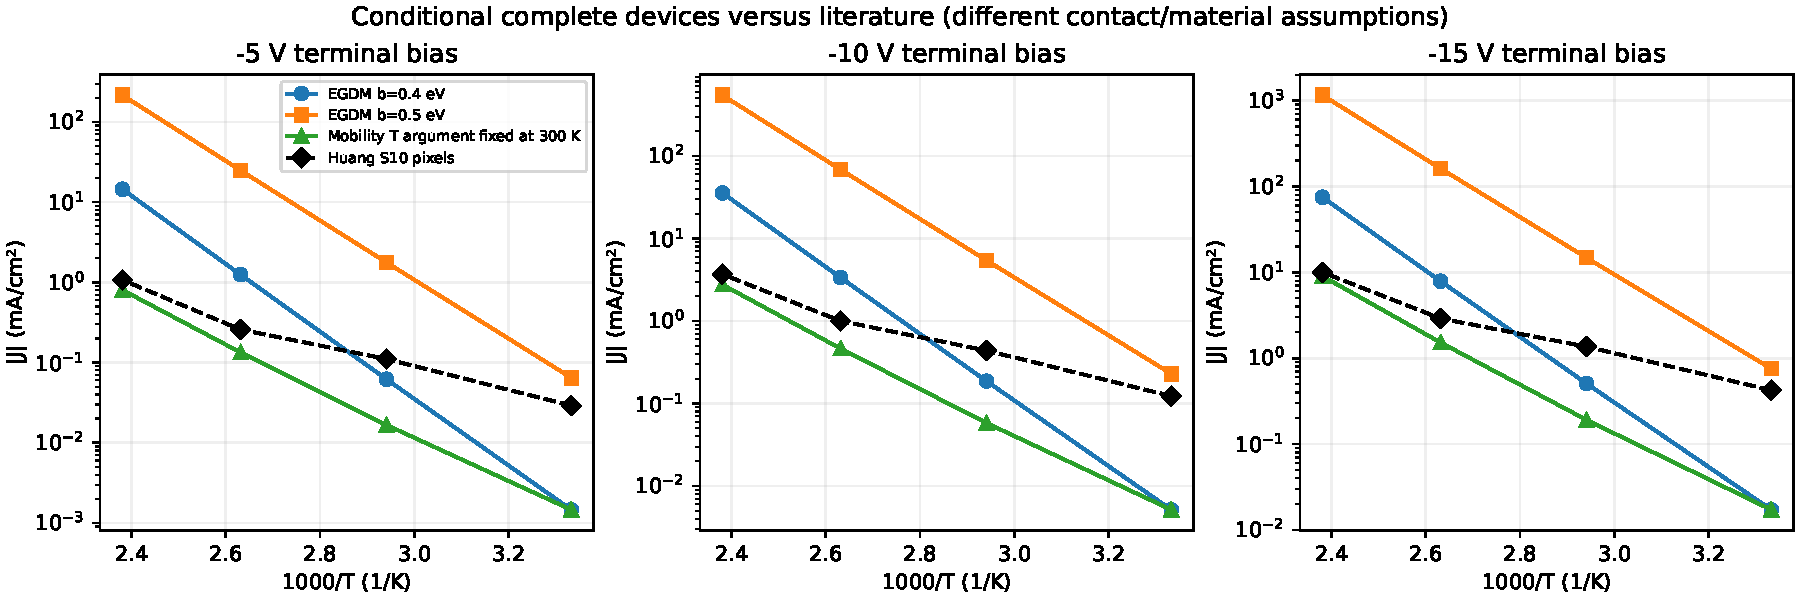
\includegraphics[width=.98\linewidth]{figures/temperature_device_comparison.pdf}
\caption{{\cjkfont 共享参数下完整器件与}\allowbreak{} Huang S10 {\cjkfont 读图对照。两个接触情景均具有过强的温度响应。文献点为数字化估计，模型线为等温条件预测；曲线不代表同一材料样品的拟合。}\allowbreak{}}
\end{figure}

\subsection{{\cjkfont 迁移率影响必须与电流来源同时分账}\allowbreak{}}
{\cjkfont 为辨认迁移率显式温度依赖的影响，控制计算只把}\allowbreak{} $\mu(n,F,T)$ {\cjkfont 中的温度参数固定为}\allowbreak{} 300 K{\cjkfont ，同时仍在实际温度下计算高斯占据、扩散热力学、反应核和接触供给。每一点重新联立求解，允许密度与场变化；这不是简单给端电流乘一个迁移率比，也不是另一种真实材料。}\allowbreak{}300 K {\cjkfont 的控制与完整模型严格相同。}\allowbreak{}

\begin{table}[htbp]\centering\small
\begin{tabular}{rrrrr}\toprule
$V$ (V)&$E_a$ {\cjkfont 完整}\allowbreak{}&$E_a$ {\cjkfont 冻结}\allowbreak{} $\mu$ {\cjkfont 温度}\allowbreak{}&420 K {\cjkfont 电流比}\allowbreak{}&$J_{\rm net\,gen}/|J|$\\\midrule
$-5$&0.8325&0.5699&18.07&$6.01\times10^{-4}$\\
$-10$&0.8000&0.5676&12.95&$2.86\times10^{-4}$\\
$-15$&0.7581&0.5659&8.30&$2.05\times10^{-4}$\\\bottomrule
\end{tabular}
\caption{$b=0.4$ eV {\cjkfont 的自洽控制。激活能单位}\allowbreak{} eV{\cjkfont ；电流比为完整模型除以只冻结迁移率显式温度的控制。最后一列在}\allowbreak{} 420 K {\cjkfont 比较净体产生折算电流与端电流。}\allowbreak{}}
\end{table}

{\cjkfont 这些情景的端电流远大于净体产生积分，说明主要是电极到电极泄漏。迁移率温度依赖确实显著影响端口响应，但拟合得到的激活能不能叫作陷阱发射势垒，也不能用来验证}\allowbreak{} Marcus {\cjkfont 产生主导。相反，在体产生受限且收集充分的极限，}\allowbreak{}$J\simeq q\int G\,dx${\cjkfont ，迁移率变化可以主要体现为密度与空间电荷调整，未必同幅改变端电流。两个极限必须由来源分账辨别。}\allowbreak{}

\begin{figure}[htbp]\centering
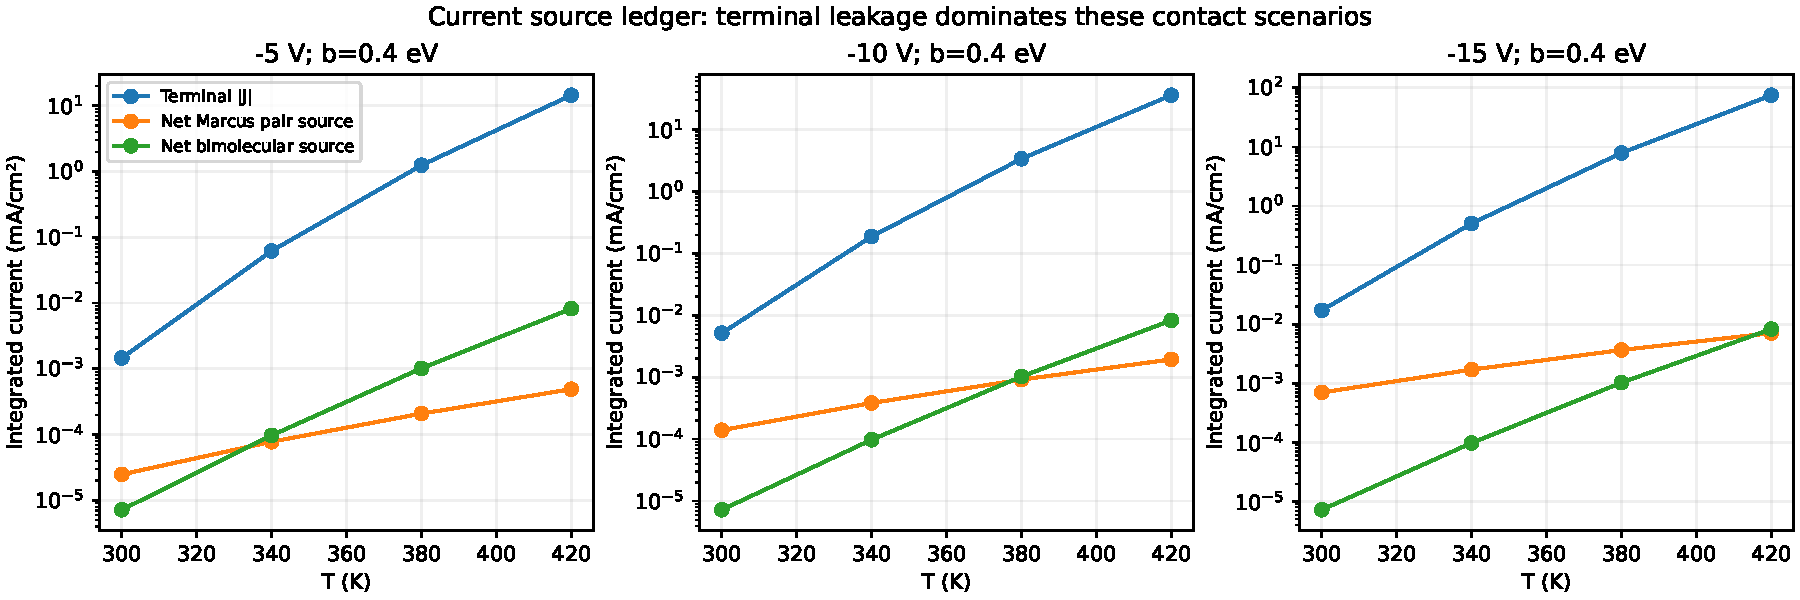
\includegraphics[width=.98\linewidth]{figures/source_current_ledger.pdf}
\caption{{\cjkfont 端电流与体产生来源分账，以及冻结迁移率温度的自洽控制。曲线之间的差别包括随输运变化而重新分布的载流子和电场，不是可逐项线性相加的独立激活能。}\allowbreak{}}
\end{figure}

\subsection{{\cjkfont 独立材料参数与数值可信范围}\allowbreak{}}
Hosseini {\cjkfont 等在另一组}\allowbreak{} PM6:BTP-eC9 {\cjkfont 器件中由变温}\allowbreak{} SCLC {\cjkfont 与高斯无序模型报告：室温零场}\allowbreak{} $\mu_n=4.1\times10^{-4}${\cjkfont 、}\allowbreak{}$\mu_p=2.1\times10^{-4}\,\mathrm{cm^2\,V^{-1}\,s^{-1}}${\cjkfont ，}\allowbreak{}$\sigma_n=53${\cjkfont 、}\allowbreak{}$\sigma_p=60$ meV{\cjkfont 。该文}\allowbreak{} 80 nm {\cjkfont 厚度只属于其自己的样品，不能赋给}\allowbreak{} Huang S10{\cjkfont 。}\allowbreak{}Huang {\cjkfont 对应器件使用}\allowbreak{} PEDOT:PSS {\cjkfont 与}\allowbreak{} PFN-Br/Ag{\cjkfont ；用户暂定}\allowbreak{} D18:L8-BO {\cjkfont 与}\allowbreak{} PDINN{\cjkfont ，界面也不同。}\allowbreak{}

{\cjkfont 仅比较低密度零场温度项，本轮}\allowbreak{} 100 meV {\cjkfont 无序和系数}\allowbreak{} 0.42 {\cjkfont 给出}\allowbreak{} $\mu(420)/\mu(300)=21.72${\cjkfont ；独立文献的系数}\allowbreak{} 0.44 {\cjkfont 与}\allowbreak{} 53/60 meV {\cjkfont 则给出}\allowbreak{} 2.47/3.19{\cjkfont 。过强温度响应因此提示同时重新约束无序和接触。但直接将}\allowbreak{} 53/60 meV {\cjkfont 代入当前}\allowbreak{} EGDM {\cjkfont 全表达式，会使部分温区}\allowbreak{} $\sigma/k_BT<2${\cjkfont ，超出已确认的密度拟合窗；高场系数也尚未核验，不能无依据补齐。}\allowbreak{}

{\cjkfont 主情景的}\allowbreak{} 24 {\cjkfont 个温度与接触工况完成}\allowbreak{} 81{\cjkfont 、}\allowbreak{}161{\cjkfont 、}\allowbreak{}321 {\cjkfont 节点检查，后两者端电流最大变化}\allowbreak{} 0.2401\%{\cjkfont 。}\allowbreak{}420 K{\cjkfont 、}\allowbreak{}$b=0.4$ eV {\cjkfont 三个反偏点进一步细化到}\allowbreak{} 641 {\cjkfont 节点，较}\allowbreak{} 321 {\cjkfont 节点分别改变}\allowbreak{} 0.0626\%{\cjkfont 、}\allowbreak{}0.0802\%{\cjkfont 、}\allowbreak{}0.0932\%{\cjkfont ；冻结迁移率温度的}\allowbreak{} $-15$ V {\cjkfont 控制改变}\allowbreak{} 0.1569\%{\cjkfont 。包括平衡点和控制，共保存}\allowbreak{} 140 {\cjkfont 个状态。最短移动电荷热力学屏蔽长度约}\allowbreak{} 3.53 nm{\cjkfont ；本轮接触情景没有此前的高占据和高场越界，但适用域通过仍不等于材料验证。}\allowbreak{}

{\cjkfont 所有状态检查连续性、非局域内部电流、}\allowbreak{}Poisson {\cjkfont 电荷、正耗散与详细平衡；公共化学势下平衡净流和净产生为零。高斯积分从}\allowbreak{} 128 {\cjkfont 增至}\allowbreak{} 256 {\cjkfont 点的端电流变化约不超过}\allowbreak{} $2\times10^{-8}${\cjkfont ，但固定状态高阶连续性缺陷可略超过求解器}\allowbreak{} $10^{-8}$ {\cjkfont 门限，因此整体精度不能用迭代残差替代。网格误差以及更大的物理参数不确定性仍是主要限制。}\allowbreak{}

{\cjkfont 本轮完整等温预测与原近欧姆接触的失败对照应并列保留。下一步先约束输运和接触，再在同一基础上更换场增强产生机制。模型没有热方程、离子、热点或损伤变量，尚不预测真实不可逆击穿，也不将可逆膝点等同失效。}\allowbreak{}

